%% sample document for AAMAS'19 conference
%%
%% modified from sample-sigconf.tex
%%
%% see ACM instructions acmguide.pdf
%%
%% AAMAS-specific questions? F.A.Oliehoek@tudelft.nl
%%

\documentclass[sigconf]{aamas}  % do not change this line!

%% your usepackages here, for example:
\usepackage{booktabs}
\usepackage{algorithmicx}
\usepackage{algorithm}
\usepackage{algpseudocode}
\usepackage{soul}
\usepackage{comment}
\usepackage{placeins}
\usepackage{color}
\usepackage{xcolor}

%% do not change the following lines
\usepackage{flushend}
\setcopyright{ifaamas}  % do not change this line!
\acmDOI{doi}  % do not change this line!
\acmISBN{}  % do not change this line!
\acmConference[AAMAS'20]{Proc.\@ of the 19th International Conference on Autonomous Agents and Multiagent Systems (AAMAS 2020), B.~An, N.~Yorke-Smith, A.~El~Fallah~Seghrouchni, G.~Sukthankar (eds.)}{May 2020}{Auckland, New Zealand}  % do not change this line!
\acmYear{2020}  % do not change this line!
\copyrightyear{2020}  % do not change this line!
\acmPrice{}  % do not change this line!

%% the rest of your preamble here


%%%%%%%%%%%%%%%%%%%%%%%%%%%%%%%%%%%%%%%%%%%%%%%%%%%%%%%%%%%%%%%%%%%%%%%%%%%%%%%%%%%%%%%%%%%%%%%%%%%%%%%%%

\begin{document}

\title{An Active Learning Method for the Comparison of Agent-based Models}  % put your title here!
%\titlenote{Produces the permission block, and copyright information}

% AAMAS: as appropriate, uncomment one subtitle line; check the CFP
%\subtitle{Extended Abstract}
%\subtitle{Blue Sky Ideas Track}
%\subtitle{JAAMAS Track}
%\subtitle{Demonstration}
%\subtitle{Doctoral Consortium}

% AAMAS: submissions are anonymous for most tracks
\author{Paper \#1775}  % put your paper number here!

%% example of author block for camera ready version of accepted papers: don't use for anonymous submissions
%
%\author{Ben Trovato}
%\authornote{Dr.~Trovato insisted his name be first.}
%\orcid{1234-5678-9012}
%\affiliation{%
%  \institution{Institute for Clarity in Documentation}
%  \streetaddress{P.O. Box 1212}
%  \city{Dublin} 
%  \state{Ohio} 
%  \postcode{43017-6221}
%}
%\email{trovato@corporation.com}
%
%\author{G.K.M. Tobin}
%\authornote{The secretary disavows any knowledge of this author's actions.}
%\affiliation{%
%  \institution{Institute for Clarity in Documentation}
%  \streetaddress{P.O. Box 1212}
%  \city{Dublin} 
%  \state{Ohio} 
%  \postcode{43017-6221}
%}
%\email{webmaster@marysville-ohio.com}
%
%\author{Lars Th{\o}rv{\"a}ld}
%\authornote{This author is the
%  one who did all the really hard work.}
%\affiliation{%
%  \institution{The Th{\o}rv{\"a}ld Group}
%  \streetaddress{1 Th{\o}rv{\"a}ld Circle}
%  \city{Hekla} 
%  \country{Iceland}}
%\email{larst@affiliation.org}
%
%\author{Valerie B\'eranger}
%\affiliation{%
%  \institution{Inria Paris-Rocquencourt}
%  \city{Rocquencourt}
%  \country{France}
%}
%\author{Aparna Patel} 
%\affiliation{%
% \institution{Rajiv Gandhi University}
% \streetaddress{Rono-Hills}
% \city{Doimukh} 
% \state{Arunachal Pradesh}
% \country{India}}
%\author{Huifen Chan}
%\affiliation{%
%  \institution{Tsinghua University}
%  \streetaddress{30 Shuangqing Rd}
%  \city{Haidian Qu} 
%  \state{Beijing Shi}
%  \country{China}
%}
%
%\author{Charles Palmer}
%\affiliation{%
%  \institution{Palmer Research Laboratories}
%  \streetaddress{8600 Datapoint Drive}
%  \city{San Antonio}
%  \state{Texas} 
%  \postcode{78229}}
%\email{cpalmer@prl.com}
%
%\author{John Smith}
%\affiliation{\institution{The Th{\o}rv{\"a}ld Group}}
%\email{jsmith@affiliation.org}
%
%\author{Julius P.~Kumquat}
%\affiliation{\institution{The Kumquat Consortium}}
%\email{jpkumquat@consortium.net}
%
%% The example's default list of authors is too long for headers
%\renewcommand{\shortauthors}{B. Trovato et al.}


\begin{abstract}  % put your abstract here!
We develop a methodology for comparing two or more agent-based models that are developed for the same domain, but may differ in the particular data sets (e.g., geographical regions) to which they are applied, and in the structure of the model. Our approach is to learn a response surface in the common parameter space of the models and compare the regions corresponding to qualitatively different behaviors in the models. As an example, we develop an active learning algorithm to learn phase transition boundaries in contagion processes in order to compare two agent-based models of rooftop solar panel adoption.
\end{abstract}


\keywords{agent-based modeling; active learning; response surface methods; model comparison}  % put your semicolon-separated keywords here!

\maketitle


%%%%%%%%%%%%%%%%%%%%%%%%%%%%%%%%%%%%%%%%%%%%%%%%%%%%%%%%%%%%%%%%%%%%%%%%%%%%%%%%%%%%%%%%%%%%%%%%%%%%%%%%%
%% start of main body of paper

\section{Introduction}

%%\begin{itemize}
%%    \item Complex large-scale agent-based models are becoming more common, in several application areas.
%%    \item These models are data-driven and specific, customized to answer specific questions or model specific phenomena.
%%    \item Often, we see multiple models for the same general phenomenon, such as epidemic spread, technology adoption, disaster evacuation, etc., created with different parameters, data sources, and model structure.
%%    \item This raises the general question of how to compare such models~\cite{axtell96aligning,burton99validation}.
%%    \item For example, in the case of the adoption of rooftop solar panels by households in two different parts of the country, we might wish to know whether it is somehow easier to have a large number of adoptions in one region than another, or whether it is just a chance difference.
%%    \item In this paper, we present a general framework to make these types of model comparisons. Then we present a specific example of the application of this framework to the comparison of two different models of the adoption of rooftop solar panels by households in two different regions of the United States.
%%    \item The rest of this paper is organized as follows. First we present the general methodological framework. Then we describe the two models we are comparing. In this specific case, model comparison requires learning a phase transition boundary in a contagion model. However, since the agent-based simulations are expensive (time-consuming) to run, we develop an active learning method with the simulation in the loop. After describing this method in detail, we present results from computational experiments with the two models. We end with a discussion of related work and future directions.
%%\end{itemize}

Complex large-scale agent-based models (ABM) are becoming increasingly common, in a huge number of application areas,
such as public health \cite{epi}, infrastructure systems such as transportation and power, disaster evacuation, and
technology adoption.
ABMs are designed to answer specific questions within an application, and their design is data-driven.
As a result, there can be multiple ABMs with a similar overall structure, but differences in the
specific model components, their interactions and parameters.
This raises the general question of how to compare such models~\cite{axtell96aligning,burton99validation}.
Axtell et al.~\cite{axtell96aligning} were the first to address this question, and developed the ``docking'' technique,
which involves verifying whether or not the dynamical properties of one ABM can be regenerated by another.
However, this is computationally intractable as ABMs become complex, and a very restrictive notion.
This question is analogous to phase space equivalence of dynamical systems \cite{ref}.

In this paper, we present a general and more scalable framework to make these types of comparisons between ABMs.
Then we present a specific example of the application of this framework to the comparison of two different 
models of the adoption of rooftop solar panels by households in two different regions of the United States.
A question of interest for local governments and utilities is to
understand who will adopt solar, and how to increase adoption.
We compare two different ABMs, one developed for California \cite{zhang16solar},
and the other for Virginia~\cite{hu19rooftop}. The probability of adoption by a household depends on a number of factors,
including demographics and characteristics of the house, as well as \emph{peer effects}, captured by the number of
households who have adopted within a 1-4 mile range. The two models have a large fraction of common factors,
but some which are distinct, e.g., pool ownership, which is a factor in the ABM of~\cite{zhang16solar},
but not in that of~\cite{hu19rooftop}. The datasets used in the calibration of these two ABMs have different
characteristics, with a much larger adoption rate in California.
In order to compare these two ABMs, we study whether it is somehow easier to have a large number of adoptions 
in one region than another, or whether it is just a chance difference. 
Our contributions are summarized below.
\begin{itemize}
\item
We design a general methodological framework based on the response surface method. We introduce a notion of
\emph{characteristic distribution} of an ABM in terms of phase space properties, e.g., phase transitions
in specific metrics. 
Finally, we design a machine learning approach based on active learning for quantitatively comparing two ABMs.
Active learning helps us reduce the number of times the simulation has to be run.
Our approach is different from direct phase space equivalence type approaches of~\cite{axtell96aligning},
and instead compares approximate representations of the phase spaces of the ABMs. Thus, this is a much
more scalable approach for complex ABMs.
\item
We illustrate our approach on the two ABMs for comparing solar adoption.
We formalize model comparison as learning a phase transition boundary in a contagion model. However, since the agent-based simulations are expensive (time-consuming) to run, we develop an active learning method with the simulation in the loop. 
Our results:
\end{itemize}

\noindent
\textbf{Organization.}
The rest of this paper is organized as follows. First we present the general methodological framework
(Section \ref{sec:framework}).
Then we describe the two models we are comparing (Section \ref{section:rooftop}).
After describing this method in detail (Section \ref{sec:learning}), we present results from computational experiments with the two models (Section \ref{sec:experiments}). We end with a discussion of related work and future directions.

\section{Framework}

Response surface methodology~\cite{box51response,carley04response}, also known as metamodel-based methods~\cite{barton06metamodel} for stochastic simulations is generally used for optimization~\cite{neddermeijer00response} and calibration~\cite{fadikar17emulation, lamperti18calibration}.
The general idea is to approximate the stochastic objective function (the ``response'') by a low order polynomial function
of the independent variables) over a part of the domain.
RSM typically runs in phases. The process starts with a screening experiment, which identifies a subset of
candidate variables, which are most significant in the region of interest.
Next, a first-order model is used to approximate the response, and a line search is used to 
find an improving direction for the objective.
In the second phase, a second-order model is used to approximate the objective, since
usually a response surface has curvature near the optimum.


We denote the agent-based simulation model as a stochastic function, $F(\xi_1, \xi_2, ..., \xi_k)$, of its parameters, assuming a fixed initial condition. In response surface methodology, we generally fit the expected value of this function,
\begin{equation}
f(\xi_1, \xi_2, ..., \xi_k) = \mathbf{E}(F(\xi_1, \xi_2, ..., \xi_k)),
\end{equation}
where $F$ is the stochastic output, given parameters $\xi_1, \xi_2, ..., \xi_k$, and $\mathbf{E}$ denotes expectation. This is appropriate when the goal is optimization or calibration.

However, when we are using the ABM to model a specific observed phenomenon, as is the case in the scenarios described in Section~\ref{section:rooftop}, the real-world data represent only one stochastic realization of the model.
Therefore, instead of taking the expectation, we characterize the behavior of the ABM in terms of the probability of seeing a particular output given a particular
parameter setting. For ease of exposition, we assume that the simulation outputs one continuous variable, $y$, though the
formalism generalizes straightforwardly to multiple outputs. We relate $y$ to the parameters as follows.
\begin{equation}
P(y_{low} < y < y_{high}) = \int P(y_{low} < F < y_{high}|\Xi)P(\Xi),
\label{eqn:output_probability}
\end{equation}
where $\Xi = [\xi_1, \xi_2, ..., \xi_k]$, and $P(\Xi)$ is a prior probability over the parameter space. Thus, the ABM can be
characterized as a discretized probability distribution, using a set of bins denoted by their bin boundaries, $\{[y_0,y_1], [y_1,y_2], ..., [y_{n-1}, y_n]\}$.
The choice of bins depends on the domain of the model. For example, models of contagion processes exhibit sharp
transitions, which are a natural choice for bin boundaries in that case, as we will see in the experiments section. We
refer to this distribution as the \emph{characteristic distribution} for the ABM.

We define the \emph{characteristic distance} between two ABMs as the distance between their characteristic distributions.
\begin{equation}
d(F_1, F_2) := D(P_1(y), P_2(y)).
\end{equation}
There are multiple valid choices for $D$, such as the (symmetric) KL-divergence, mean-squared distance, total variation distance, earth-mover's distance, etc. Note that this distance is well-defined even if the two ABMs have entirely different parameter spaces, since it is defined only over the output space. Thus it is a fairly general method of comparison. 
For a given observed value, $y_{obs}$, we can also directly compare the 
probabilities assigned by the two models to the corresponding bin.
\begin{equation}
    d_{obs}(F_1, F_2) := P_1(B_{obs}) - P_2(B_{obs}),
\end{equation}
where $B_{obs}$ is the bin within which $y_{obs}$ lies. This directly tells us how much more likely it is to see $y_{obs}$ in one model versus the other.

For a general comparison of the two ABMs in the case where the two ABMs have an overlap in their parameter space (i.e., they have some parameters in common), we can have a more detailed comparison. Let $\Xi_{c}$ be the parameters that the two ABMs have in common. We can partition this subspace of the parameter space into regions based on the most likely bin for $y$ for each parameter setting.
\begin{equation}
    B(\Xi_{c}) = \argmax_B \int_{\Xi \setminus \Xi_{c}} P(B|\Xi)P(\Xi \setminus \Xi_{c}),
\label{eqn:B}
\end{equation}
where $B$ denotes a bin, corresponding to the bin boundaries defined earlier, and $\Xi \setminus \Xi_{c}$ denotes the parameters other than the common parameters. The equation above assigns to each point in the common parameter subspace, a bin corresponding to the most likely output at that point.

Now we define the \emph{disagreement}, $\Delta$, between the two ABMs as the probability of choosing a parameter setting, according to the prior distribution, that results in a difference in the outputs of the two models.
\begin{equation}
    \Delta(F_1, F_2) = \int_{\Xi_{c}} \mathbf{1}(B_1(\Xi_{c}), B_2(\Xi_{c}))P_1(\Xi_{c}),
\end{equation}
where $\mathbf{1}(B_1(\Xi_{c}), B_2(\Xi_{c}))$ is an indicator function that is 1 if $B_1(\Xi_{c}) = B_2(\Xi_{c})$ and 0 otherwise. $\Delta$ gives the total probability, over the subspace $\Xi_c$, that the outputs of the two ABMs will fall into different bins. Note that $\Delta$ is a directed measure, since $\Delta(F_1, F_2) \ne \Delta(F_2, F_1)$.

There are various ways to compute the integral in equation~\ref{eqn:B}. The typical approach in simulation
science is to use adaptive experiment designs [CITE]. Here we propose a machine learning approach based on active learning. The general idea is to train a multi-class classifier, where a class corresponds to a bin, for each model. Since the simulations can often be expensive to run, an active learning approach can help minimize the number of times the simulation has to be run.
The classifiers are used to estimate $B(\Xi_{c})$ for each ABM.
Once the classifiers have been trained, we can use them to estimate $\Delta$.

The active learning approach to training the classifier involves running the simulation in a loop with the classifier. In each round, the simulation is run to generate additional labeled points for the classifier. Then the classifier is trained on the updated data set and we do uncertainty sampling [CITE] in the parameter space to generate new parameter settings where the simulation is to be evaluated in the next round. The process stops when the labels generated by the simulation agree with the labels generated by the classifier.
\section{Rooftop Solar Panel Adoption}
\label{section:rooftop}
We compare two ABMs for rooftop solar adoption, one built by Zhang et al. for San Diego, California~\cite{zhang16solar} and the other for Shenandoah Valley region in Virginia, as described below in Section~\ref{sec:virginia_model}. They both use a set of demographic, social, economic and geographical variables to assess the probability of adoption for each household in respective study areas. A logistic regression model is built in each case to identify important factors that influence solar adoption. These factors are then used by their respective ABMs to study the diffusion of adoption. Since the solar penetration rate in Virginia is much smaller compared to California, a decision-adjusted logistic regression model was used to handle the issue of class imbalance in Virginia.

\begin{table}[H]
	\centering
	\caption{Features used in regression for Virginia model}
	\begin{tabular}{|l|p{5cm}|}
		\hline
		{\bf Feature} & {\bf Description} \\ 
		\hline
		acreage & Acreage of the house. \\ 
		\hline
		area\_type & Rural (0) or urban (1). \\ 
		\hline
		asrYear & Year house was built.  \\ 
		\hline
		baths & Num of bathrooms. \\ 
		\hline
		bedrooms & Num of bedrooms. \\ 
		\hline
		NPV & Net Present Value. \\ 
		\hline
		climateRegionPub & Type of climate. \\ 
		\hline
		dailyConsumption & Avg. electricity used in Watt
                                   hrs. \\ 
		\hline
		education & Highest education achieved. \\ 
		\hline
	    fuelheat & Type of fuel used for heat. \\ 
	    \hline
		income & Household's yearly income.  \\ 
		\hline
		numCarStorage & Num. of car storage in the house. \\
		\hline 
		sqFootage & Sq. footage of the house.  \\ 
		\hline
		swimpool & Pool present or not. \\ 
		\hline
		totalVal & Estimated house value. \\
		\hline 
		typehuq & Type of housing unit. \\ 
		\hline
		householdSize & Family size. \\ 
		\hline
		%X1Mile & Adopters within 1 mile. \\ 
		%X2Mile & Adopters within 2 mile. \\ 
		%X3Mile & Adopters within 3 mile. \\ 
		%X4Mile & Adopters within 4 mile. \\ 
		Mile1 & Adopters within 1 mile. \\ 
		Mile2 & Adopters within 2 mile. \\ 
		Mile3 & Adopters within 3 mile. \\ 
		Mile4 & Adopters within 4 mile. \\
		\hline
	\end{tabular}
	\label{tab: feature description}
\end{table}
\subsection{The Virginia Model} \label{virginia_model}

We build a statistical model to identify features that contribute to a household's decision to adopt rooftop solar panels.
However, due to low penetration of solar adopters in rural regions, the data on
solar adopters is sparse, which makes it difficult to build a good
prediction model. Given highly imbalanced training data, traditional statistical methods
tend to predict most households to be non-adopters in order to minimize
the mis-classification error and provide high overall prediction
accuracy.

In our study, we are more interested in identifying potential adopters
so we apply a decision-adjusted modeling approach 
from Mao et al.~\cite{Mao}, and Hu et al.~\cite{hu19rooftop}. The decision-adjusted
approach optimizes the prediction model with respect to a user-stated
evaluation criterion. We set this criteria to maximize the sum of True
Positive Rate and True Negative Rate. The decision-adjusted approach can be applied to
different statistical models, here we choose logistic regression model as
our baseline model.

The decision-adjusted solar adopter prediction model is as
follows. Suppose a prediction model is obtained from data
$\{X_i,I_i(\delta),Y_i\}_{i=1}^n$, where $X_i$ are the demographic features as
shown in Table~\ref{tab: feature description}.  $Y_i$ is the response,
$Y_i = 1$ means household is an adopter and $Y_i = 0$ means non-adopter, $I_i(\delta)$ are the indicator features for corresponding demographic features, which is defined as
\begin{equation*}
I_i(\delta)=\left\{
\begin{array}{@{}ll@{}}
1, & \text{if }X_i > \delta;\\
0, & \text{if }X_i \leq \delta,
\end{array}\right.
\end{equation*}

The indicator features are introduced when the coefficients of linear combination are not able to
capture all information in the model. For example, if the coefficient of a feature
is positive, then a larger value of the feature will increase the
likelihood of adoption. However, this positive relationship may not be
constant; it may be strong when the value of the
feature is small, and weak when the value of the feature is
large. The indicator features address this issue.

The logistic regression model has the link function below,
\begin{align*}
\text{Pr}(Y=1|X, I(\delta))=\frac{exp\Big(\big(X, I(\delta)\big)^T\beta\Big)}{1+exp\Big(\big(X, I(\delta)\big)^T\beta\Big)}
\end{align*}
Where $\beta$ is the regression coefficient. For the logistic regression with elastic net, $\beta$ is estimated through maximizing a penalized log-likelihood $l(\beta)-P(\beta,\alpha,\lambda)$, where 
\begin{align*}
P(\beta,\alpha,\lambda)=\lambda\big((1-\alpha)\frac{1}{2}||\beta||_2^2+\alpha||\beta||_1\big)
\end{align*}


The predicted label for this household is determined by the following, where $\tau$ is the threshold probability for determining whether a household is adopter or not. 
\begin{equation*}
\hat{Y_i}=\hat{Y_i}(X_i,I_i(\delta),\alpha,\lambda,\tau)=\left\{
\begin{array}{@{}ll@{}}
1, & \text{if Pr}(Y_i=1)\ge \tau \\
0, & \text{if Pr}(Y_i=1)< \tau
\end{array}\right.
\end{equation*}
Then the optimization problem for our decision-adjusted model is
\begin{equation*}
\max_{\delta,\alpha,\lambda,\tau} \Omega\Big(\hat{Y_i}(X_i,I_i(\delta),\alpha,\lambda,\tau),Y\Big)
\end{equation*}
Where $\Omega(\cdot)$ is a function of predicted label
$\hat{Y_i}(X_i,I_i(\delta),\alpha,\lambda,\tau)$, and true label
$Y$. It is determined by the specific goals of the study, as defined
by the user. 

In the decision adjusted model, we want to maximize ($\Omega=$
TPR$+$TNR) given $\tau$ and $\delta$. Here `TPR' refers to true
positive rate, `TNR' refers to true negative rate, `FP' refers to false positives, and `FN' refers to false negatives. The TPR$+$TNR is defined as:

%\begin{equation*}
%\Omega=\text{TPR}+\text{TNR}=\frac{TP}{TP+FN}+\frac{TN}{TN+FP}.
%\end{equation*}

\begin{equation*}
            \Omega=\frac{TP}{TP+FN}+\frac{TN}{TN+FP}=\frac{TP}{Condition\ positives}+\frac{TN}{Condition\ negatives},
        \end{equation*}

This is an improvement over accuracy as the performance matrix, which
is given by:

\begin{equation*}
        \text{ACCURACY}=\frac{TP+TN}{TP+FN+TN+FP}=\frac{TP+TN}{n}.
        \end{equation*}


Table \ref{tab: model coefficients} summarizes the model results. The climateRegion, education, fuelheat, type of housing unit are categorical features, the coefficient for each level are shown in the table.

The tuning paraments selected from the decision-adjusted approach are: \\
$\bullet$ $\tau = 0.0022$, a household with predicted probability greater than 0.0022 is classified as an adopter.\\
$\bullet$ $\lambda = 0.000303$, $\alpha = 0.4$, which are values of tuning parameters in enet penalty.\\
$\bullet$ $\delta(\text{totalVal}) = 75000$, if the value of feature totalVal is greater than 75000, then the value of the corresponding indicator feature is 1.\\

\begin{table}[H]
	\centering
	\scriptsize
    \caption{Virginia model features and the corresponding coefficients.}
	\begin{tabular}{|p{6cm}|r|}
		\hline
		Variable & Coefficient \\ 
		\hline
		\hline
		intercept & -10.6 \\ 
		\hline
		acreage & -0.123 \\ 
		\hline
		area\_type & -1.79 \\ 
		\hline
		asrYear & 0.00184 \\
		\hline 
		baths &    0 \\ 
		\hline
		bedrooms & 0.0881 \\ 
		\hline
		dailyConsumption & 5.65e-07 \\ 
		\hline
		income &    0 \\ 
		\hline
		NPV &    0 \\ 
		\hline
		numCarStorage & 0.331 \\ 
		\hline
		sqFootage &    0 \\ 
		\hline
		swimpool & 0.169 \\ 
		\hline
		totalVal & -3.66e-07 \\  
		\hline
		householdSize & 0.123 \\ 
		\hline
		\textbf{climateRegion} & \\
		PubCold/Very Cold & -1.09 \\ 
		Hot-Humid & 0.00883 \\ 
		Mixed-Humid &    0 \\ 
		\hline
		\textbf{education} & \\
		Less than high school diploma or GED & 0 \\
		High school diploma or GED  & -0.0117 \\ 
		Some college or Associate’s degree  & 0.332 \\ 
		Bachelor’s degree  &    0 \\ 
		Masters, Professional, or Doctorate degree  &    0 \\ 
		\hline
		\textbf{fuelheat} & \\
		Natural gas from underground pipes  & 0 \\ 
		Propane (bottled gas)  & -0.528 \\ 
		Fuel oil/kerosene  & 0.269 \\ 
		Electricity  &    0 \\ 
		Wood  & 0.472 \\ 
		\hline
		\textbf{Type of housing unit} & \\
		Mobile home  & 0 \\
		Single-family detached house  & 0.00162 \\ 
		Single-family attached house  & -0.479 \\
		\hline
		\textbf{Neighborhood feature} & \\
		%X1Mile & 0.399 \\ 
		%X2Mile &    0 \\ 
		%X3Mile & 0.0299 \\ 
		%X4Mile & 0.0376 \\ 
		Mile1 & 0.399 \\ 
		Mile2 &    0 \\ 
		Mile3 & 0.0299 \\ 
		Mile4 & 0.0376 \\
		\hline
		Indicator feature for totalVal & -1.12 \\ 
		\hline
	\end{tabular}
	\label{tab: model coefficients}
\end{table}
\subsection{The San Diego Model}


The San Diego model was developed by Zhang et al.~\cite{zhang16solar}. The model was trained on extensive data collected to the California Solar Initiative \url{https://www.gosolarcalifornia.ca.gov/about/csi.php}. In addition, property assessment data for San Diegor county and electricity utilization data for participants in the rebate program was collect (energy utilization data as limited to the 12 months before adoption). The data set spanned 6 years and 8500 adopters and included detailed information about the solar panel purchasing decision, including the system size, reported cost, incentive, whether the system was purchased or leased and date of adoption.

The ABM developed from this data used machine learning techniques to train an individual model of solar panel adoption behavior. Individuals agents changed their behavior based on household characteristics, seasons and peer-effects. \cite{zhang16solar} provides details on the specific variables used and the results. 

For this work we used the model provided here: \url{https://github.com/haifeng-zhang/ddabm-solar} which focused on modeling a single zipcode within the San Diegor region. For this work we used the model provided here: \url{https://github.com/haifeng-zhang/ddabm-solar} which focused on modeling a single zipcode within the San Diegor region. 


\section{Model Comparison Method}
\label{sec:learning}

% {\color{magenta} Use the reference of framework section to write this scetion more formally}\\

In this section, we instantiate the framework described in Section~\ref{sec:framework} to compare the models described in Section~\ref{section:rooftop}. 
Both the Virginia model and the San Diego model are network contagion models,
where a contagion (in this case a technology: rooftop solar panels) spreads through a network. Both models belong to the general class of $SI$ contagion models,
drawn from mathematical epidemiology, where $S$ stands for $Susceptible$
and $I$ stands for $Infectious$. In our case, $Infectious$ corresponds to adopter. Once a household has adopted solar panels, their peer influence on their neighbors is assumed to persist indefinitely.
This means that, in the limit, all households in both models will be adopters, as
long as the parameters are set in such a way that the probability of adoption if at
least one neighbor has adopted is non-zero. However, depending on the parameter
settings, it can be the case that the probabilities of adoption are so low that 
we see very few adoptions in the duration for which the simulations are run. Network
structure can also play a role in speeding up or slowing down the spread of the 
contagion through the network.

As the probability of adoption increases, the SI model undergoes a phase transition,
where the simulation shows a sharp qualitative change in its behavior. As the probability of adoption crosses a threshold, the simulation quickly changes from only a few nodes being adopters to a lot (or most) of the nodes becoming adopters in a short amount of time. Due to this qualitative behavior, we choose just two bins to describe each simulation in Section~\ref{section:rooftop}, corresponding to small and large numbers of adopters. The actual values chosen are listed in Section~\ref{sec:experiments}.

Another nice aspect of this scenario is that the variance in the output of the 
simulation shows a sharp peak at the phase transition boundary, and tends to be low
away from the boundary. This is illustrated in Figure~\ref{fig:diagDisplay}. Thus, by running multiple runs of the simulation for any 
chosen point in parameter space, we get a clear signal if the point is close to the phase transition boundary. We make use of this fact in our active learning algorithm below.

In this section, we introduce an active learning~\cite{sung95active} method for learning the decision boundary. 
Figure \ref{fig:workflow} gives a general idea of the proposed methodology. The goal of the proposed method is
to learn the decision boundary that separates large breakout from small breakouts with minimum number of queries in the parameter space.

Notations used in the remainder of the paper for method description, results and discussion:\\
$start$, $end$ = the endpoints of a line in the 2D parameter search space on which binary search is performed. These points qualify as end points only if they can separate the search space into small and large outbreaks. \\
\noindent
$pMean$, $pStdev$ = mean and standard deviation of the number of adoptions across 20 replicates of the diffusion model at the last time step. In this instance, the diffusion model (or ABM) is evaluated at $p$.\\
\noindent
$evaluatedPoints$ = List of labeled points in the 2D parameter search space. A point is labeled as 0 if the mean number of adoptions is less than a certain threshold.\\
\noindent
$boundaryPoints$ = List of points in the 2D parameter search space that are close to or on the decision boundary. If the standard deviation of the number of adoptions at the point is greater than a certain threshold, then the point is classified as a boundary point.

Initially, a suitable range of the parameter search space is selected. In our experiments, the search space is instantiated with two parameters. 
A seed labeled dataset is created from the search space to train the classifier the first time. 
Binary search is performed across the diagonal of the parameter space to find a potential boundary point, followed by querying neighboring points of such a boundary point with uncertainty sampling.
% TODO: Roughly 5-10 points are labeled -> this means how much % of data is labeled for first training of the classifier. 
% Why we look for variacne of the point - describe that in 1 sentence
The classifier is then trained on this seed dataset.

Further iterations generate more labeled data by intelligently querying unlabeled instances in the parameter search space by employing uncertainty sampling technique.
To find potential boundary points, the algorithm exploits the knowledge gained in terms of the decision boundary, $evaluatedPoints$, and $boundaryPoints$ in the parameter space. To choose the next set of endpoints to perform binary search, a point $start$, is chosen such that it is close to or on the current decision boundary, but far away from existing $boundaryPoints$ and $evaluatedPoints$ in the search space. 
Evaluate the ABM outcome at $start$ in terms of $sMean$ and $sStdev$. The $end$ point is chosen from $evaluatedPoints$ such that, it is the farthest point from $start$ and with an opposite label of the $start$ point. Points are queried in the search space until the termination condition is reached.
% Roughly how much % of points is queried at the end as compared to the area of the search space

%Once the point is queried, mean and standard deviation are used to evaluate the role of the queried point. If a point is found to be potentially very close to/on the boundary, then, the classifier is trained on the incremental set of labeled points. The knowledge of the latest decision boundary also influences the choice of unlabeled point tp be queried.




\begin{algorithm}

\caption{Active learning for predicting decision boundary}
\label{alg:methodAlgo}
\begin{algorithmic}[1]

\State $Input$ : $DiffusionModel$,
2D search space for parameters $p1,p2$ 
\State $Output$ : $evaluatedPoints$ , $boundaryPoints$

\Procedure{LearnDecisionBoundary}{}
    \State $start$  = $[p1Min, p2Min]$
    \State $end$  = $[p1Max, p2Max]$
    \State $[boundaryPt, bMean, bStdev] = \Call{BinarySearch}{start,end}$
    \State \Call{EvaluateNearbyPoints}{$boundaryPt$} Add these points to $evaluatedPoints$
    \State $noRounds$ = 1
    \While{$noRounds < = 5$}
        \State \textbf{\textit{$nextPt$}} = \Call{GetNextPointViaActiveLearning}{}
        \State $[nextPt, nMean, nStdev]$ = \Call{RunDiffusionModel}{$nextPt$}
        \If{$nStdev >= STDEV-THRESHOLD$ }
            \State Add $nextPt$ to $boundaryPoints$
        \Else 
            \State Add $[nextPt, nMean, nLabel]$ to $evaluatedPoints$
        \EndIf
        \State $oppositePt$ = Another point with label opposite to $nLabel$ and farthest from $nextPt$
        \State $[boundaryPt, bMean, bStdev] = \Call{BinarySearch}{nextPt,oppositePt}$
        \State \Call{EvaluateNearbyPoints}{$boundaryPt$} Add these points to $evaluatedPoints$
        
        \State $noRounds++$
        
     \EndWhile
    
    \State return \textbf{$evaluatedPoints$ , $boundaryPoints$}

\EndProcedure
\end{algorithmic}
\end{algorithm}


\begin{algorithm}[H] {
\caption{Binary search to find a potential boundary point}
\label{alg:binSearch}
\begin{algorithmic}[1]
\Procedure{BinarySearch}{$pt_1, pt_2$}
    \State $[pt_1Mean, pt_1Stdev]$ = \Call{RunDiffusionModel}{$pt_1$}
    \If{$pt_1Stdev >= STDEV-THRESHOLD$ }
            \State Add $pt_1$ to $boundaryPoints$
            \State return \textbf{[$pt_1, pt_1Mean, pt_1Stdev$]}
        \Else 
            \State Add $[pt_1,pt_1Mean,pt_1Label]$ to $evaluatedPoints$
    \EndIf
    \State $[pt_2Mean, pt_2Stdev]$ = \Call{RunDiffusionModel}{$pt_2$}
    \If{$pt_2Stdev >= STDEV-THRESHOLD$ }
            \State Add $pt_2$ to $boundaryPoints$
            \State return \textbf{[$pt_2, pt_2Mean, pt_2Stdev$]}
        \Else 
            \State Add $[pt_2,pt_2Mean,pt_2Label]$ to $evaluatedPoints$
    \EndIf
    \State $m = (pt_1 + pt_2)/2.0$ 
    \While{ $m \notin boundaryPoints$ and $pt_1Label \neq pt_2Label$}
        \State $[mMean, mStdev]$ = \Call{RunDiffusionModel}{$m$}
        \If{$mStdev >= STDEV-THRESHOLD$ }
            \State Add $m$ to $boundaryPoints$
            \State return \textbf{[$m, mMean, mStdev$]}
        \Else 
            \State Add $[m,mMean,mLabel]$ to $evaluatedPoints$ 
        \EndIf
        \State Assign $m$ to $pt_1$ or $pt_2$, s.t. $pt_1$ and $pt_2$ have different labels
        \State $m = (pt_1 + pt_2)/2.0$ 
    \EndWhile
\EndProcedure
\end{algorithmic}
}
\end{algorithm}
\section{Experiments}

Experiments are done with two agent based models in three regions with different population sizes. Number of agents in each of the region are as follows: Rappahannock county has 2495 agents, San Diego has 12925 agents, Shenandoah Valley Region (SVR) has 138043 agents. 

\begin{figure}
    \centering
    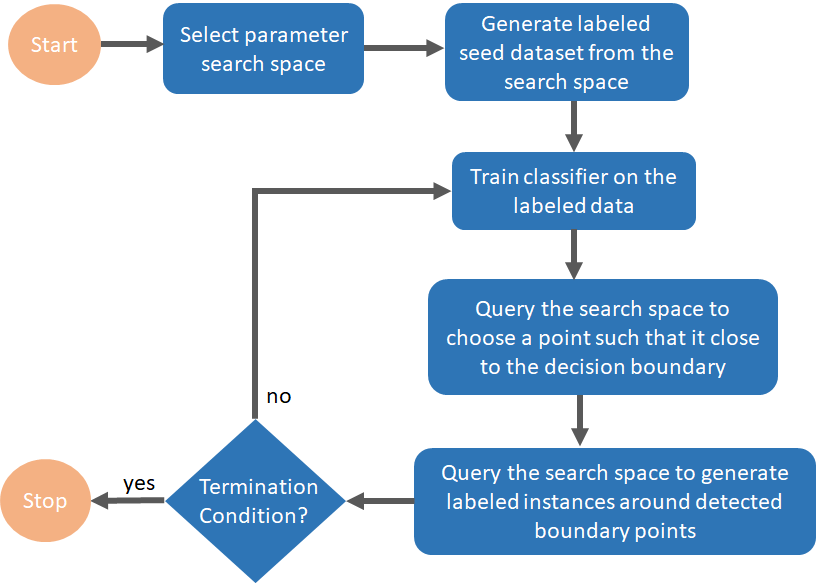
\includegraphics{AAMAS20Template-submission/figures/workflow.png}
    \caption{Overview of the presented methodology - A common set of parameters is chosen from both ABMs and an active learning framework is implemented to learn the decision boundary that separates small and large solar panel adoptions. }
    \label{fig:workflow}
\end{figure}

Both the agent-based diffusion models simulate the number of households adopting rooftop solar.
The model presented in Section \ref{virginia_model} is used for Rappahannock county in Virginia and Shenandoah Valley Region in Virginia. 
The model presented in Section \ref{san-diego-model} is used for San Diego.
In order to facilitate comparison between the 2 ABMs, we choose to explore the common parameters in both the models: Mile1 and NPV. All experiments are conducted in 2D space using Mile1 and NPV.

Before learning the decision boundary that separates the low and high adoptions for the three regions, we need to set the parameter extents of the search space, $STDEV-THRESHOLD$ for boundary point condition, and $MEAN-THRESHOLD$ for labeling points evaluated in the search space. Diffusion model outputs are examined for points across the diagonal of an arbitrary parameter space. As an example, Figures \ref{fig:diagmean}, \ref{fig:diagstdev}, and \ref{fig:diagDisplay} show the output of the ABMs in terms of mean and standard deviation. On observing the sharp transitions in mean and standard deviation, $STDEV-THRESHOLD$ is set to 250 and $MEAN-THRESHOLD$ is set to 1000 for Rappahannock. Similar experiments are performed for SVR and San Diego regions to set the thresholds.
In all the experiment settings and results shown, the ABM results are averaged over 20 replicates to calculate mean and standard deviation. 
%If time out happens then we discard the point or process how many every replicates are completed.
{\color{magenta} Q for Samarth: Should we give the mean and stdev thresholds for each region?}

\begin{figure}
    \centering
    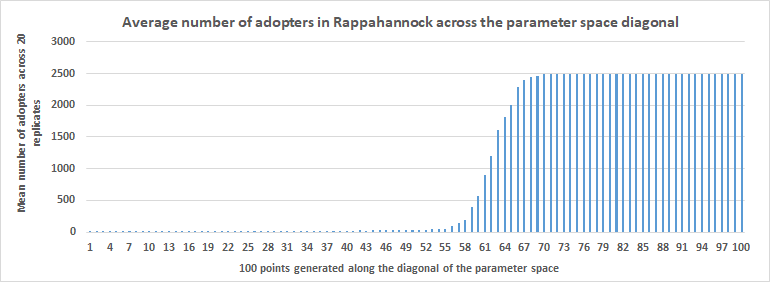
\includegraphics{AAMAS20Template-submission/figures/rapp-diag-mean1.png}
    \caption{Diagonal Mean <ADD MORE>}
    \label{fig:diagmean}
\end{figure}

\begin{figure}
    \centering
    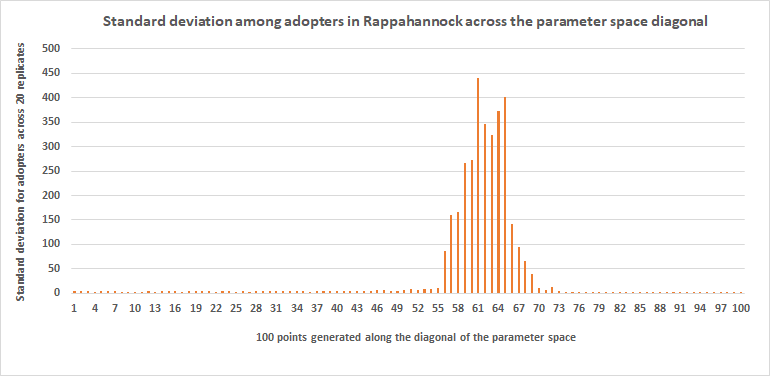
\includegraphics{AAMAS20Template-submission/figures/rapp-diag-stdev1.png}
    \caption{Diagonal Stdev <ADD MORE>}
    \label{fig:diagstdev}
\end{figure}

\begin{figure}
\begin{subfigure}{.25\textwidth}
  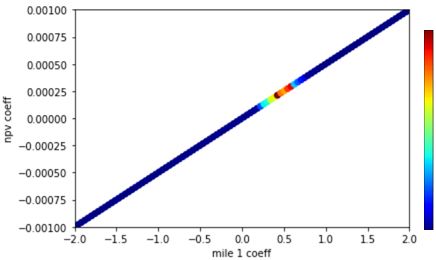
\includegraphics[height=3cm,width=4cm]{AAMAS20Template-submission/figures/rapp100diagstdev1.png}
    %\caption{Standard deviation for points on diagonal}
  %\label{fig:diagstdev}
\end{subfigure}%
\begin{subfigure}{.25\textwidth}
  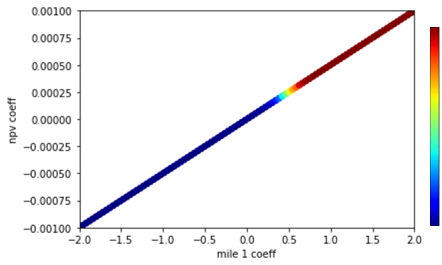
\includegraphics[height=3cm,width=4cm]{AAMAS20Template-submission/figures/rapp100diagmean1.png}
  %\caption{Mean for points on diagonal}
  %\label{fig:}
\end{subfigure}
\caption{Standard deviation and mean for points evaluated by ABM on the diagonal of the 2D search space. The colors blue to red represent transition from small outbreak to large outbreak. Some variability is observed for both mean and standard deviation between 0.3 to 0.6 on the x-axis which denotes the range for mile 1 coefficient. When seen in reference to Figure \ref{fig:diagRappMean} and Figure \ref{fig:diagRappStdev} this region shows a sharp transition from small outbreak to large outbreak.}
\label{fig:diagDisplay}
\end{figure}

\begin{comment}
\begin{figure}
    \centering
    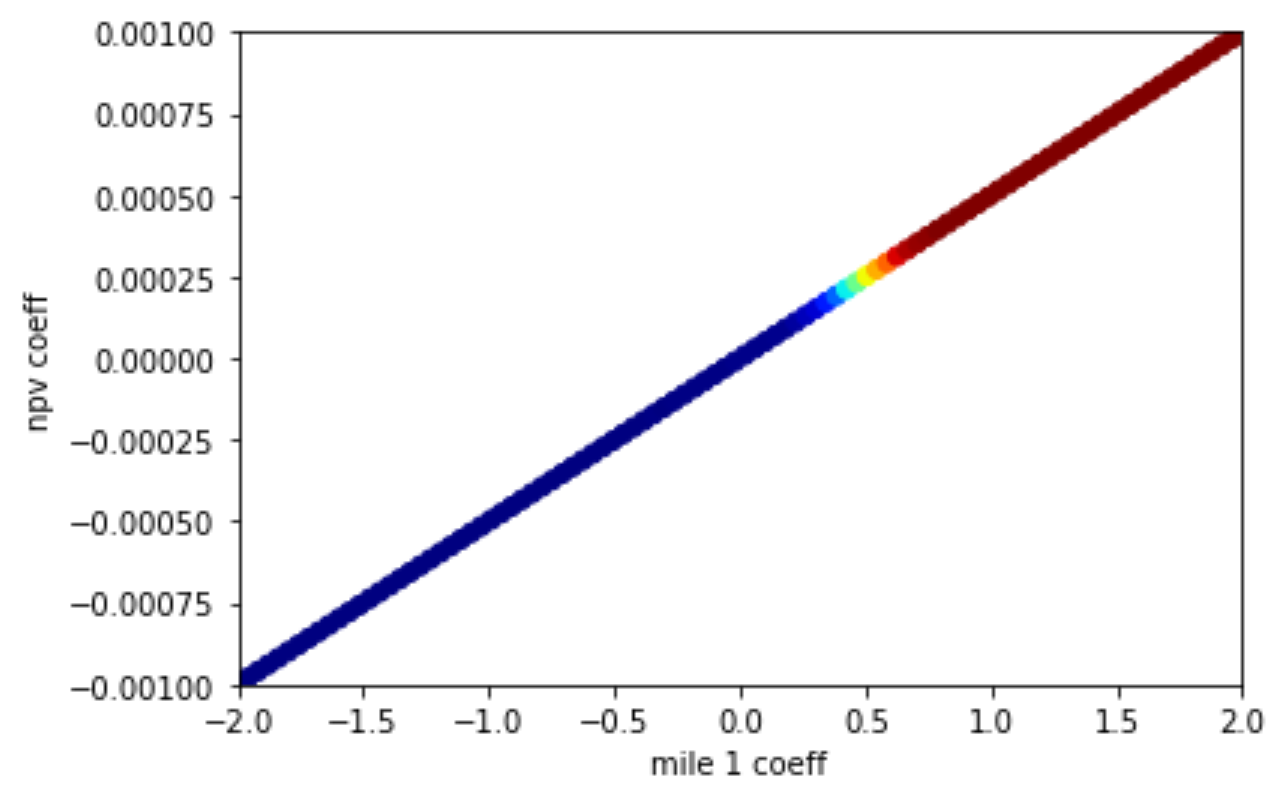
\includegraphics[height=3cm,width=4cm]{AAMAS20Template-submission/figures/rapp100diagmean.png}
    \caption{Diagonal Mean <ADD MORE>}
    \label{fig:diagRappMean}
\end{figure}

\begin{figure}
    \centering
    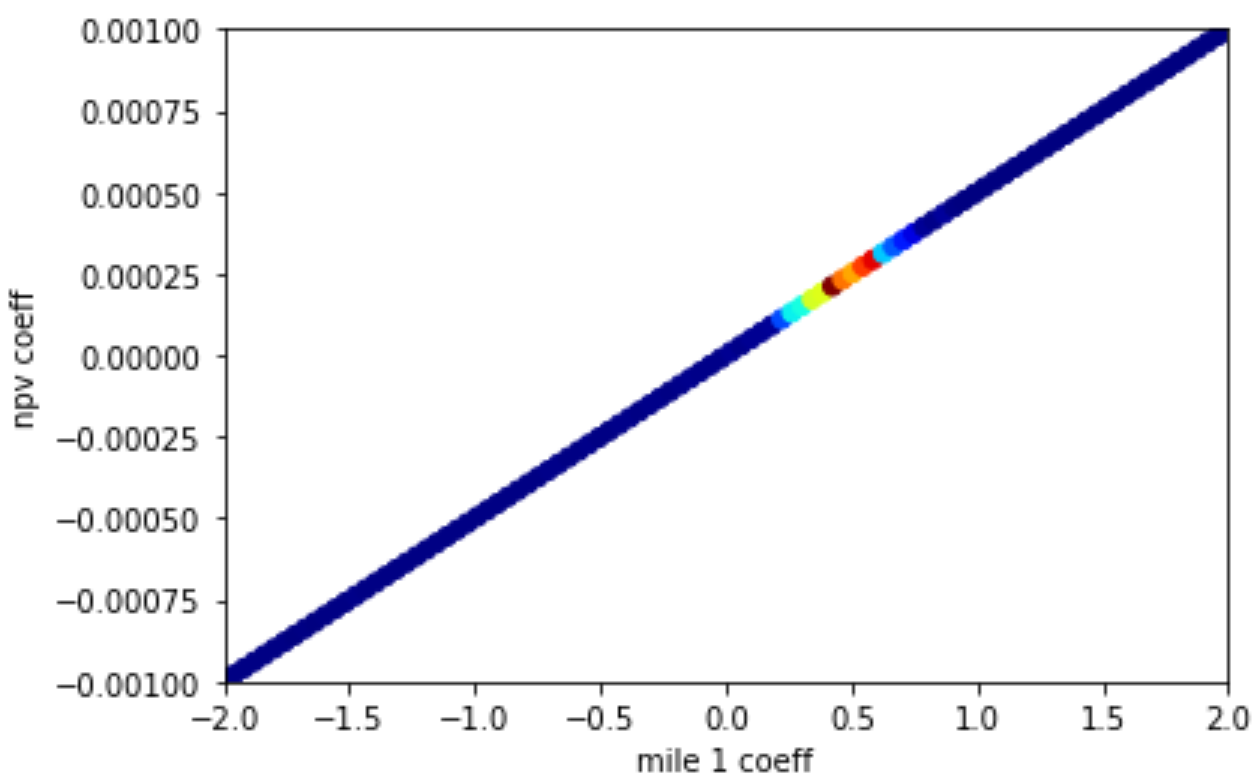
\includegraphics[height=3cm,width=4cm]{AAMAS20Template-submission/figures/rapp100diagstdev.png}
    \caption{Diagonal Stdev <ADD MORE>}
    \label{fig:diagRappStdev}
\end{figure}
\end{comment}

Once the thresholds are set, we conduct three sets of experiments:\\
1. Model \ref{virginia_model} for Rappahannock county\\
2. Model \ref{virginia_model} for SVR region\\
3. Model \ref{san-diego-model} for a zipcode in San Diego\\
First, the search space is initialized with the seed set generation. Classifier is trained on this initial labeled data.
In successive rounds of learning, every time a boundary point is found by binary search, a fixed number of points are queried and labeled in the neighborhood of the boundary point. These labeled points are used to train the classifier in every round.

In order to initiate a binary search that leads to meaningful generation of boundary point, two types of approaches are tried for each set of experiments. These approaches are used to find a start point for binary search. The first set of endpoints is chosen to be the diagonal of the parameter search space. From the next round, points are chosen intelligently by exploiting the knowledge of $boundaryPoints$ and $evaluatedPoints$.\\
First Approach:
Use SVM linear classifier and generate points near/on the SVM linear boundary.
Choose one point from this set that is far away from existing points in $evaluatedPoints$ and $boundaryPoints$.\\
Second approach:
Train Random Forest classifier with $evaluatedPoints$. Then, query points in the search space such that their neighbors collectively have roughly equal distribution pf labels indicating that they are close to the boundary. Choose one point from this set that is far away from existing points in $evaluatedPoints$ and $boundaryPoints$.\\


\section{Results}
\section{Related Work}
\section{Discussion}

The method is extendable to any classifier. We tried Random forest and SVM linear kernel.
We propose two strategies for choosing points close to or on the decision boundary but far away from the $boundaryPoints$ and $evaluatedPoints$ in the search space. Neighbor points and svm line equation.

How many points is enough points to learn the boundary? Do we have an explainable heuristic?

Do we have any metric to show that?

Do we reduce the number of runs of the diffusion model to learn the decision boundary?



\bibliographystyle{ACM-Reference-Format}  
\bibliography{mc-bibliography}  

\end{document}
